\chapter{Supplementary material}

%\resp{Franco Aquistapace Tagua}
% TASK 6
\section{Song-Havlin-Makse self-similar model}
\label{sec:SHM_SM}
 
\subsubsection*{Algorithmic implementation of the renormalisation procedure}
The renormalisation of a given network is performed algorithmically as follows:

\begin{enumerate}
	\item Initialise a box with a randomly picked node.
	\item For every remaining node $i$, add it to the box if $\max_{j\in B} d(i,j) \leq L_B$, where $B$ contains the nodes currently in the box, and $d(i,j)$ is the shortest path between nodes $i$ and $j$.
	\item Repeat steps 1. and 2. with the remaining available nodes until all nodes are assigned to a box.
\end{enumerate}

\subsubsection*{Correlation profiles}

The correlation profile $R(k_1, k_2) = P(k_1, k_2) / P_r(k_1, k_2)$ is defined as the ratio between the joint degree--degree probability distribution of the network of interest, $P(k_1, k_2)$, and the joint degree--degree probability distribution of a randomised uncorrelated version of the same network, $P_r(k_1, k_2)$, where the links have been randomly rewired while preserving the degree distribution. 

In this work, the joint degree--degree probability distribution is estimated in a frequentist approach, by considering all equivalent instances as observations. For example, to obtain $P(k_1, k_2)$ for the minimal model graph with $e=1.0$, the degree--degree pairs of the 10 graphs generated for $e=1.0$ are collected. Then, the joint probability for a given pair $(k_1, k_2)$ is calculated as in Eq. \ref{eq:P_joint_task_6_SM}:

\begin{equation}
	P(k_1, k_2) = \frac{N_{obs}(k_1, k_2)}{N_{obs, tot}} \ \ ,
	\label{eq:P_joint_task_6_SM}
\end{equation}
where $N_{obs}(k_1, k_2)$ is the number of occurrences of the pair $(k_1, k_2)$, and $N_{obs, tot}$ is the total number of observations. The same methodology is applied for the calculation of $P_r(k_1, k_2)$. No interpolation is done for pairs $(k_1', k_2')$ that are not observed, and their probability is thus taken as $P(k_1', k_2') = 0$.


\subsubsection*{Scaling relations}

The descriptor $N_B(L_B) / N$ is defined as the ratio between the number of original nodes, $N$, and the number of boxes, $N_B$, obtained after performing a renormalisation step with box size $L_B$. Meanwhile, the descriptor $\mathcal{S}(L_B) = k_B(L_B) / k_{hub}$ is the ratio between the maximum degree of the boxes after a renormalisation step with box size $L_B$, $k_B(L_B)$, and the maximum degree of the among the original nodes, $k_{hub}$. For both scaling relations, $N_B(L_B) / N$ and $\mathcal{S}(L_B)$, the mean value and standard deviation is obtained for each $L_B$ from the 10 networks generated for both cases $e=1.0, 0.8$. From the obtained results, the theoretical models proposed in the source material \cite{song2006origins} are fitted. 

For the fractal case $e=0.8$, $N_B(L_B) / N$ and $\mathcal{S}(L_B)$ are described, respectively, by Eqs. \ref{eq:N_fractal_SM} and \ref{eq:S_fractal_SM}:

\begin{equation}
	N_B(L_B) / N = C_N (L_B + L_0)^{-d_B}
	\label{eq:N_fractal_SM}
\end{equation}

\begin{equation}
	\mathcal{S}(L_B) = C_S (L_B + L_0)^{-d_k}
	\label{eq:S_fractal_SM}
\end{equation}
where $L_0$, $d_B$, $d_k$, $C_N$ and $C_S$ are parameters fitted from the data. The data points with $L_B < 8$ were excluded from the fit of $N_B(L_B) / N$, and those with $L_B < 12$ were excluded from the fit of $\mathcal{S}(L_B)$. From the fit, the values $d_B = 2.83$ and $d_k = 2.91$ are obtained. 

On the other hand, for the non--fractal case $e=1.0$, $N_B(L_B) / N$ and $\mathcal{S}(L_B)$ are described, respectively, by Eqs. \ref{eq:N_non_fractal_SM} and \ref{eq:S_non_fractal_SM}:

\begin{equation}
	N_B(L_B) / N = C_N \exp(-L_B / L_0)
	\label{eq:N_non_fractal_SM}
\end{equation}

\begin{equation}
	\mathcal{S}(L_B) = C_S \exp(-L_B / L_0)
	\label{eq:S_non_fractal_SM}
\end{equation}
where again $L_0$, $C_N$ and $C_S$ are fitted from the data. In this case, the data points with $L_B > 12$ are excluded from the fit of both $N_B(L_B) / N$ and $\mathcal{S}(L_B)$.



% TASK 15
\section{Sandpile dynamics on complex networks}
\label{sec:SOC_SM}

% BTW explainer
\subsubsection*{Bak-Tang-Wiesenfeld sandpile model simulations}

In general, for each avalanche event in the Bak-Tang-Wiesenfeld model simulations, the following quantities are registered:
\begin{itemize}
	\item Avalanche area, $A$: defined as the number of distinct nodes participating in an avalanche event.
	\item Avalanche size, $S$: defined as the number of toppling events in a given avalanche.
	\item Number of toppled grains, $G$.
	\item Avalanche duration, $T$.
	\item Bulk avalanche status, $B$: defined as a boolean value that indicates if no grains are lost during the avalanche.
\end{itemize}

For the simulations on interdependent networks the following observations are additionally registered: subgraph where an avalanche originates, local size of the avalanche in the origin subgraph and inflicted size of the avalanche on the non-origin subgraph.

% Scale-free networks
\subsubsection*{Generation of scale--free networks}

In this work, the static model from \cite{goh2003sandpile} is used to generate scale--free networks with desired properties as follows. First, a set of $N$ nodes is indexed as $i=1,..., N$ and are assigned a weight $w_i=i^{-\alpha}$, where $\alpha\in[0,1)$ controls the degree distribution of the network as $\gamma=1 + 1/\alpha$, for large $N$. Then, in an iterative manner, two nodes $i$ and $j$ are selected with relative probabilities $w_i$ and $w_j$, and an edge is created between them if no edge is already present. This process is repeated until the average degree of the network is $\langle k\rangle=2m$. Here, the networks are generated with $2\times10^5$ nodes, $m=2$ leading to an average degree $\langle k\rangle=4$, and degree exponents $\gamma=2.01, 2.2, 2.4, 2.6, 2.8, 3.0, 5.0, \infty$.

In order to avoid spurious effects in the sandpile simulations, isolated nodes and possibly other small subgraphs are removed from the system by only keeping the largest connected component. In general, the amount of removed nodes is not significant when compared to the size of the remaining network.

\subsubsection*{Characterisation of avalanches in scale--free networks}

The distribution of the area of bulk avalanches in the simulations performed on scale--free networks, $P_a(A)$, is modelled here by Eq. \ref{eq:P_A_tau_def}:

\begin{equation}
	P_a(A) = C A^{-\tau} \exp(-A / s_c) \ ,
	\label{eq:P_A_tau_def}
\end{equation}
where $C$ and $\tau$ are fitted from the data, and the avalanche characteristic size is set as $s_c=(\langle k\rangle f)^{-1}$. In order to fit the model, the observations for $A$ are first binned logarithmically using $N_{bins}=13$ bins, and the first $N_{skip}=3$ bins are excluded from the fit. It is noted in this work that the choice of $N_{bins}$ and $N_{skip}$ has a significant impact on the resulting values for $\tau$, and the results presented here are the ones closest to the theoretical prediction from the branching process approach. 

On the other hand, the relationship between the bulk avalanche size $S$ and the duration $T$ is defined by Eq. \ref{eq:S_vs_T_scalefree_def}:

\begin{equation}
	S = C_z T^z \ ,
	\label{eq:S_vs_T_scalefree_def}
\end{equation}
where $C_z$ and $z$ are fitted from the data. To fit Eq. \ref{eq:S_vs_T_scalefree_def}, the data outside of a range $(T_{min}, T_{max})$ is discarded. The values $T_{min}$ and $T_{max}$ are chosen so as to isolate the range in $T$ where the model holds. 

Fig. \ref{fig:SM_scale_free_distributions} presents $P_a(A)$ with respect to $A$, and $S$ with respect to $T$ for the bulk avalanches registered in simulations on the scale--free networks. The results are presented for the cases $\gamma=2.01, 2.2, 3.0, \infty$. The best fits of Eqs. \ref{eq:P_A_tau_def} and \ref{eq:S_vs_T_scalefree_def}, respectively, are also shown. The simulation results for $P_a(A)$ are presented after logarithmic binning, and only the mean values of $S$ for each unique value of $T$ are shown.

\begin{figure}[!h]
	\begin{center}
	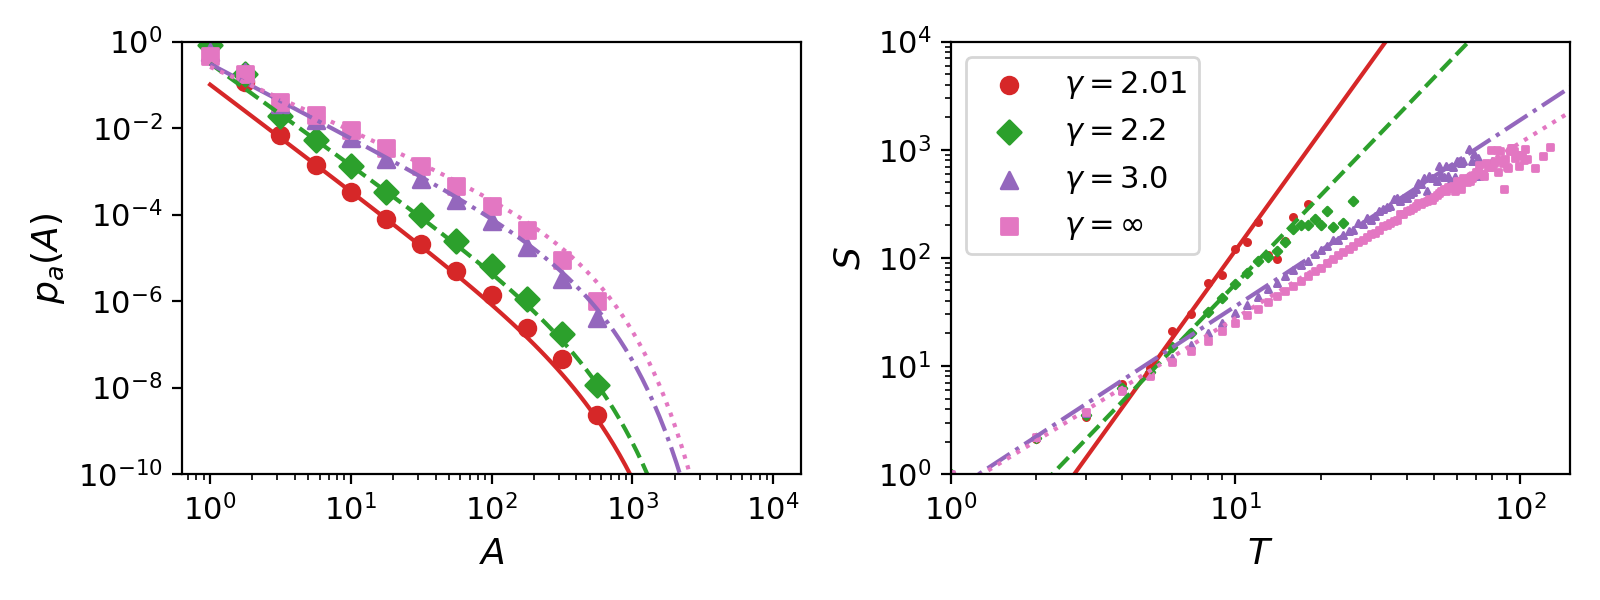
\includegraphics[scale=0.75]{./images/task_15/SM_scale_free_distributions.png} 
	\end{center}
	\caption{Distribution of avalanche area, $P_a(A)$, (left) and avalanche size, $S$, with respect to duration, $T$, (right) for bulk avalanches. The results for simulations on scale--free networks with degree exponent $\gamma=2.01,2.2,3.0,\infty$ are shown, as well as the best fit of the theoretical models. To increase clarity, only the mean value of $S$ for each unique value of $T$ is shown for each case, and the marker size for data points $(S,T)$ is reduced. \\} 
	\label{fig:SM_scale_free_distributions} 
\end{figure}


\subsubsection*{Generation of interdependent regular networks}

In this work, each interdependent network is first initialised as two separate $z$-regular subgraphs, $G_A$ and $G_B$, with uniform degree $z=3$ and $2\times10^3$ nodes each. Then, the connection between these subgraphs is done by means of uncorrelated Bernoulli coupling, as follows: for each node in $G_A$ a random number is uniformly sampled from $(0,1)$, if that number is smaller than a threshold $p$ then an available node from $G_B$ is uniformly sampled and a link to it is established. The selected node from $G_B$ is then removed from the set of available nodes, so that each node in $G_A$ can be connected at most to a single node from $G_B$, and vice versa. In order to cover a wide but detailed range of $p$, a network is generated for each value in $p=0.001, 0.005, 0.01, 0.025, 0.05, 0.075, 0.1, 0.15, 0.2, 0.3, 0.4, 0.5$.


\subsubsection*{Characterisation of avalanches in interdependent networks}

A large avalanche is here defined as an avalanche with size $S > N' / 2$, where $N'$ is the amount of nodes in a single subgraph of the system. Additionally, the quantity $N_{X}^Y(S_{large})$ is defined as the amount of large avalanches measured in $Y$ which originated in $X$, where $X,Y\in\{A, B\}$. Then, the probability of a large local avalanche, $P_{local}(S_{large})$, is defined by Eq. \ref{eq:P_local_S_large_def}:

\begin{equation}
	P_{local}(S_{large}) = \frac{1}{2}\left(\frac{N_A^A(S_{large})}{N^A} +\frac{N_B^B(S_{large})}{N^B}\right) \ ,
	\label{eq:P_local_S_large_def}
\end{equation}
where $N^A$ and $N^B$ are the total number of avalanches observed in $A$ and $B$, respectively, regardless of their origin. On the other hand, the probability of a large inflicted avalanche, $P_{inf}(S_{large})$, is defined as in Eq. \ref{eq:P_inf_S_large_def}:

\begin{equation}
	P_{inf}(S_{large}) = \frac{1}{2}\left(\frac{N_A^B(S_{large})}{N^B} +\frac{N_B^A(S_{large})}{N^A}\right) \ .
	\label{eq:P_inf_S_large_def}
\end{equation}
Finally, the global probability of a large avalanche, $P_{global}(S_{large})$, is defined by Eq. \ref{eq:P_global_S_large_def}:

\begin{equation}
	P_{global}(S_{large}) = \frac{P_{local}(S_{large}) + P_{inf}(S_{large}) }{2} \ .
	\label{eq:P_global_S_large_def}
\end{equation}

Another relevant factor when considering interconnected systems is the size of the largest avalanches in the entire network. In this work, it is noted that such size is directly related to the coupling probability $p$. This is displayed in Fig. \ref{fig:SM_large_avalanche_rank_plot_joint_AB} as a rank plot of the size $S$ for the $10^3$ largest avalanches, for $p=0.001, 0.01, 0.1$. It can be seen that an increase in $p$ leads to an increase $S$ for the largest avalanches in the system, in agreement to what is reported in the reference material \cite{brummitt2012suppressing}.


\begin{figure}[!h]
	\begin{center}
	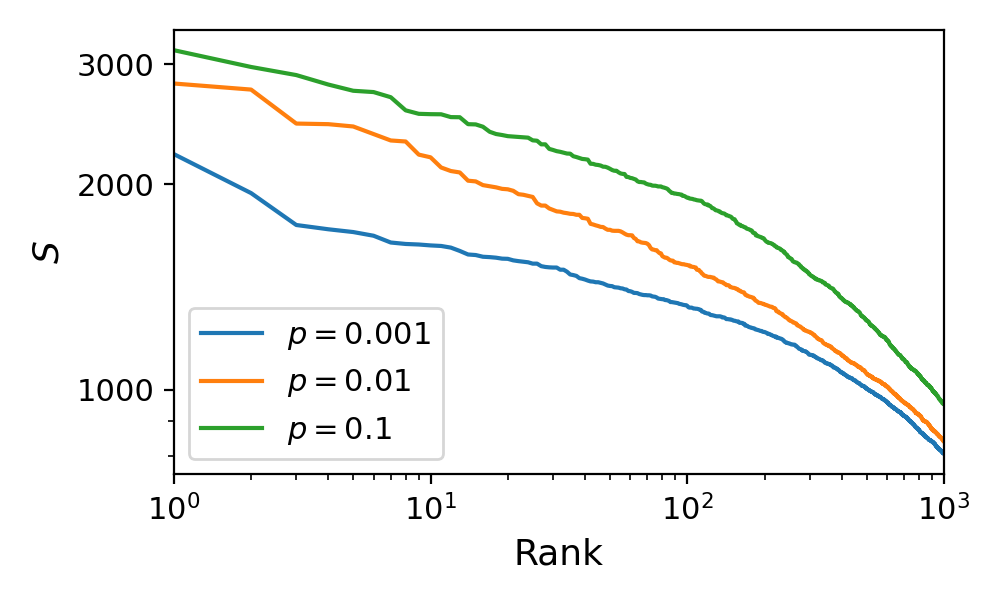
\includegraphics[scale=0.75]{./images/task_15/SM_large_avalanche_rank_plot_joint_AB.png} 
	\end{center}
	\caption{Rank plot of the avalanche size, $S$, for the $10^3$ largest avalanches in interdependent networks. Results are presented for the cases $p=0.001, 0.01, 0.1$. \\} 
	\label{fig:SM_large_avalanche_rank_plot_joint_AB} 
\end{figure}



\newpage